\documentclass[border=10pt]{standalone}
\usepackage{tikz}

\usepackage{amssymb} %maths
\usepackage{amsmath} %maths
\usepackage[utf8]{inputenc} %utile pour taper directement les caractères accentués

\begin{document}

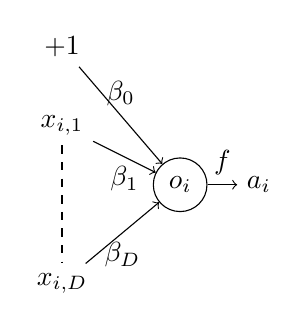
\begin{tikzpicture}
    \node[draw, circle] (oi) at  (1.5,1.25) {$o_i$};
    \node (offset) at  (0,3) {$+1$};
    \node (xi1) at  (0,2) {$x_{i, 1}$};
    \node (xid) at  (0,0) {$x_{i, D}$};
    \node (ai) at  (2.5,1.25) {$a_i$};

    \draw[->] (offset) -- (oi) node[midway,above]{$\beta_0$};
    \draw[->] (xi1) -- (oi) node[midway,below]{$\beta_1$};
    \draw[->] (xid) -- (oi) node[midway,below]{$\beta_D$};
    \draw[->] (oi) -- (ai) node[midway,above]{$f$};
    \draw[dashed] (xi1) -- (xid);
\end{tikzpicture}

\end{document}
